% !TeX root = ../main.tex
\chapter{Applications of the differential calculus}

\lettrine{T}{h}e various notions which were introduced in the previous chapter are useful for some applications.
This is what we explore in this chapter.


\section{Partial differential equations}

There are a huge number of different types of partial differential equations and here we consider here just a few types.

\subsubsection*{First order linear PDEs}


\begin{example*}
    Find all solutions of the partial differential equation
    \(3 \frac{\partial f}{\partial x}(x,y) + 2 \frac{\partial f}{\partial y} (x,y) = 0\).

    \solution
    \begin{enumerate}
        \item Equivalent to
              \(\left( \begin{smallmatrix}
                  3 \\ 2
              \end{smallmatrix} \right)
              \cdot
              \nabla f(x,y) =0\);
        \item Directional derivative \( D_{v}f(x,y) = 0\) where \(v=\left( \begin{smallmatrix}
                      3 \\ 2
                  \end{smallmatrix} \right)\);
        \item This means that \(f\) is constant in the direction \(\left( \begin{smallmatrix}
                  3 \\ 2
              \end{smallmatrix} \right)\);
        \item All solutions have the form \(f(x,y) = g(2x-3y)\) for some \(g:\bR \to \bR\).
    \end{enumerate}
\end{example*}



\begin{theorem}
    Let \(g:\bR\to\bR\) be differentiable, \(a,b\in \bR\), \((a,b)\neq (0,0)\).
    If \(f(x,y):= g(bx-ay)\) then
    \[
        a \frac{\partial f}{\partial x} (x,y) + b \frac{\partial f}{\partial y} (x,y) = 0.
    \]
    Conversely, every \(f\) which satisfies this equation is of the form \(g(bx-ay)\).
\end{theorem}


\begin{proof}
    \begin{description}
        \item[\((\Rightarrow\))]
              \begin{enumerate}
                  \item If \(f(x,y)= g(bx-ay)\) then, by the chain rule,
                        \(\partial_x f(x,y) = bg'(bx-ay)\) and \(\partial_y f(x,y) = -ag'(bx-ay)\).
                  \item
                        Consequently \(a\partial_x f(x,y) + b \partial_y f(x,y) = a bg'(bx-ay) - abg'(bx-ay) = 0\).
              \end{enumerate}

        \item[(\(\Leftarrow\))]
              \begin{enumerate}
                  \item Let \(\left(\begin{smallmatrix}
                                u\\ v
                            \end{smallmatrix}\right)
                        = \left(\begin{smallmatrix}
                                a & b \\ b & -a
                            \end{smallmatrix}\right)
                        \left(\begin{smallmatrix}
                                x \\ y
                            \end{smallmatrix}\right)\)
                        and so
                        \(\left(\begin{smallmatrix}
                                x\\ y
                            \end{smallmatrix}\right)
                        = \frac{-1}{a^2 + b^2} \left(\begin{smallmatrix}
                                a & b \\ b & -a
                            \end{smallmatrix}\right)
                        \left(\begin{smallmatrix}
                                u \\ v
                            \end{smallmatrix}\right)\).
                        %\item Let \(u=ax+by\), \(v=bx-ay\) and observe that \(x=\frac{au + bv}{a^2 + b^2}\) and that \(y=\frac{au + bv}{a^2 + b^2}\).
                  \item Let \(h(u,v)=f(\frac{au + bv}{a^2 + b^2}, \frac{bu-av}{a^2+b^2})\).
                  \item Calculate
                        \[
                            \partial_u h(u,v)
                            = \tfrac{1}{{a^2 + b^2}}
                            \left( a \partial_x f
                            + b \partial_y f \right)  (au + bv, bu-av) = 0.
                        \]
                  \item Namely, \(h(u,v)\) is a function of \(v\) only so take \(g(v) = h(u,v)\) and so \(f(x,y) = g(bx-ay)\).
              \end{enumerate}
    \end{description}

\end{proof}





\subsubsection*{1D wave equation}

The \emph{1D wave equation} is
\[
    \frac{\partial^2 f}{\partial x^2}(x,t) = c^2  \frac{\partial^2 f}{\partial t^2}(x,t).
\]
Here \(x\) represents the position along string,
\(t\) is time and \(f(x,t)\) is the displacement of the string from the centre at position \(x\), at time \(t\).
The constant \(c\) is a fixed parameter depending on the string.

This partial differential equation is derived from the equation of motion \(F = m a\) where \(F\) is the tension in the string, \(a\) is the acceleration from horizontal and \(m\) is the mass of a little piece of the string.
The equation is valid for small displacement.
In this case the \emph{boundary conditions} are natural: Are the ends of the string fixed? Is only one end fixed? At time \(t=0\), is the string already moving?

\begin{theorem}
    Let \(F\) be a twice differentiable function and \(G\) a differentiable function.
    \begin{enumerate}
        \item
              Then the function defined as
              \begin{equation}
                  \label{eq:wave}
                  f(x,t) = \frac{1}{2}(F(x+ct) + F(x-ct)) + \frac{1}{2c} \int_{x-ct}^{x+ct} G(s) \ ds
              \end{equation}
              satisfies \(   \frac{\partial^2 f}{\partial x^2}(x,t) = c^2  \frac{\partial^2 f}{\partial t^2}(x,t) \),
              \(f(x,0) = F(x)\)
              and \(\frac{\partial f}{\partial t}(x,0) = G(x)\).
        \item
              Conversely, if a solution of  \(   \frac{\partial^2 f}{\partial x^2}(x,t) = c^2  \frac{\partial^2 f}{\partial t^2}(x,t) \) satisfies
              \[\frac{\partial^2 f}{\partial x \partial t}(x,t) = \frac{\partial^2 f}{\partial t \partial x}(x,t),\]
              then it has the above form \eqref{eq:wave}.
    \end{enumerate}

\end{theorem}


\begin{proof}[Proof of part 1.]
    \begin{enumerate}
        \item Let \(f(x,t)\) be as defined \eqref{eq:wave} and calculate
              \[
                  \begin{aligned}
                      \tfrac{\partial f}{\partial x} (x,t)
                       & = \tfrac{1}{2} \left(F'(x+ct) + F'(x-ct)\right)
                      + \tfrac{1}{2c}\left(G(x+ct) - G(x-ct)\right)               \\
                      \tfrac{\partial^2 f}{\partial x^2}(x,t)
                       & = \tfrac{1}{2} \left(F''(x+ct) + F''(x-ct)\right)
                      + \tfrac{1}{2c}\left(G'(x+ct) - G'(x-ct)\right)             \\
                      \tfrac{\partial f}{\partial t} (x,t)
                       & = \tfrac{1}{2} \left(cF'(x+ct) - c F'(x-ct)\right)
                      + \tfrac{1}{2}\left(G(x+ct) + G(x-ct)\right)                \\
                      \tfrac{\partial^2 f}{\partial t^2} f(x,t)
                       & = \tfrac{1}{2} \left(c^2F''(x+ct) + c^2 F''(x-ct)\right)
                      + \tfrac{c}{2}\left(G'(x+ct) + G'(x-ct)\right)
                  \end{aligned}
              \]
        \item Observe that  \(   \frac{\partial^2 f}{\partial x^2}(x,t) = c^2  \frac{\partial^2 f}{\partial t^2}(x,t) \).
        \item Observe that \(f(x,0) = F(x)\)
              and \(\frac{\partial f}{\partial t}(x,0) = G(x)\).
    \end{enumerate}
\end{proof}


\begin{proof}[Proof of part 2.]
    \begin{enumerate}
        \item Suppose that \(f\) satisfies the 1D wave equation;
        \item Introduce \(u = x + ct\), \(v=x-ct\)
              and observe that \(x = \frac{u+v}{2}\), \(t=\frac{u-v}{2c}\);
        \item Define \(g(u,v) = f(x,t) = f(   \frac{u+v}{2} , \frac{u-v}{2c} )\);
        \item By the chain rule
              \[
                  \begin{aligned}
                      \tfrac{\partial g}{\partial u}(u,v)
                       & = \tfrac{1}{2} \tfrac{\partial f}{\partial x}(   \tfrac{u+v}{2} , \tfrac{u-v}{2c} )
                      + \tfrac{1}{2c} \tfrac{\partial f}{\partial t}(   \tfrac{u+v}{2} , \tfrac{u-v}{2c} )                      \\
                      \tfrac{\partial^2 g}{\partial v \partial u}(u,v)
                       & = \tfrac{1}{4} \tfrac{\partial^2 f}{\partial x^2}(   \tfrac{u+v}{2} , \tfrac{u-v}{2c} )
                      - \tfrac{1}{4c} \tfrac{\partial^2 f}{\partial x\partial t}(   \tfrac{u+v}{2} , \tfrac{u-v}{2c} )          \\
                       & \ \ +  \tfrac{1}{4c} \tfrac{\partial^2 f}{\partial x \partial t}(   \tfrac{u+v}{2} , \tfrac{u-v}{2c} )
                      -  \tfrac{1}{4c^2} \tfrac{\partial^2 f}{\partial t^2}(   \tfrac{u+v}{2} , \tfrac{u-v}{2c} ) = 0;
                  \end{aligned}
              \]
        \item So \( \tfrac{\partial g}{\partial u}(u,v) = \varphi_0(u)\) and \(g(u,v) = \varphi_1(u) + \varphi_2(v)\).
              I.e., \(f(x,t) = \varphi_1(x+ct) + \varphi_2(x-ct)\);
        \item Let \(F(x) := \varphi_1(x) + \varphi_2(x)\);
        \item \(F'(x) = \varphi_1'(x) + \varphi_2'(x)\)
              and \(\frac{\partial f}{\partial t}(x,t) = c\varphi_1(x+ct) - c\varphi_2(x-ct)\);
        \item Let \(G(x) := \frac{\partial f}{\partial t}(x,0) = c\varphi_1(x) - c\varphi_2(x)\).
    \end{enumerate}
\end{proof}



\section{Extrema (minima / maxima / saddle)}

Let \(S\subset \bR^n\) be open,
\(f:S \to \bR\) be a scalar field
and \(\aa \in S\).

\begin{definition}[absolute min/max]
    If \(f(\aa)\leq f(\xx)\) (resp.\ \(f(\aa)\geq f(\xx)\)) for all \(\xx \in S\), then \(f(\aa)\) is said to be the \emph{absolute} minimum (resp.\ maximum) of \(f\).
\end{definition}

\begin{definition}[relative min/max]
    If \(f(\aa)\leq f(\xx)\) (resp.\ \(f(\aa)\geq f(\xx)\)) for all \(\xx \in B(\aa,r)\) for some \(r>0\), then \(f(\aa)\) is said to be a \emph{relative} minimum (resp.\ maximum) of \(f\).
\end{definition}

Collectively we call the these points the \emph{extrema} of the scalar field.
In the case of a scalar field defined on \(\bR^2\) we can visualize the scalar field as a 3D plot like Figure~\ref{fig:bumps}.
Here we see the extrema as the ``flat'' regions.
In this setting we use \emph{global} as a synonym of \emph{absolute} and \emph{local} as a synonym of \emph{relative}.


\begin{figure}[htb]
    \centering
    \includegraphics{bumps.pdf}
    \caption{$f(x,y) := x e^{-(x^2y^2)}  + \frac{1}{4}e^{y^\frac{3}{10}}$}
    \label{fig:bumps}
\end{figure}

To proceed it is convenient to connect the extrema with the behaviour of the gradient of the scalar field.

\begin{theorem}
    If \(f:S\to\bR\) is differentiable and has a relative minimum or maximum at \(\aa\), then \(\nabla f(\aa)=  \mathbf{0}\).
\end{theorem}

\begin{proof}
    \begin{enumerate}
        \item Suppose \(f\) has a relative minimum at \(\aa\) (or consider \(-f\));
        \item For any unit vector \(\vv\) let \(g(u) = f(\aa+u\vv)\);
        \item \(g\) has relative minimum at \(u=0\) so \(u'(0)=0\);
        \item This means that \(D_{\vv} f(\aa) = 0\) for every \(\vv\) and so \(\nabla f (\aa)= \mathbf{0}\). \qedhere
    \end{enumerate}
\end{proof}



\begin{figure}[htb]
    \begin{center}
        \includegraphics{inflection.pdf}
        \caption{\(\nabla f(\aa) =  \mathbf{0}\) doesn't imply a minimum or maximum at \(\aa\) as seen for the function \(f(x):=x^3\).}
    \end{center}
\end{figure}

Observe that here and in the subsequent text, we can always consider the case of \(f:\bR \to \bR\), i.e., the case of \(\bR^n\) where \(n=1\).
Everything still holds and reduces to the arguments and formulae previously developed for functions of one variable.


\begin{definition}[stationary point]
    If \(\nabla f(\aa)=0\) then \(\aa\) is called a \emph{stationary point}.
\end{definition}


\begin{figure}[htb]
    \begin{center}
        \includegraphics[width=0.5\textwidth]{bowl.pdf}
        \caption{If \(f(x,y)=x^2+y^2\) then \(\nabla f(x,y) = \left(\begin{smallmatrix}
                2x\\2y
            \end{smallmatrix}\right)\) and \(\nabla f(0,0) =\left(\begin{smallmatrix}
                0\\0
            \end{smallmatrix}\right) \). The point \((0,0)\) is an absolute minimum for \(f\).}
    \end{center}
\end{figure}


\begin{definition}[saddle point]
    If \(\nabla f(\aa)=0\) and \(\aa\) is neither a minimum nor a maximum then \(\aa\) is said to be a \emph{saddle point}.
\end{definition}



\begin{figure}
    \begin{center}
        \includegraphics{pringle.pdf}
        \caption{If \(f(x,y)=x^2-y^2\) then \(\nabla f(x,y) = \left(\begin{smallmatrix}
                2x\\-2y
            \end{smallmatrix}\right)\) and \(\nabla f(0,0) =\left(\begin{smallmatrix}
                0\\0
            \end{smallmatrix}\right) \). The point \((0,0)\) is a saddle point for \(f\).}
    \end{center}
\end{figure}


\section{Hessian matrix}

To proceed it is useful to develop the idea of a second order Taylor expansion in this higher dimensional setting.
In particular this will allow us to identify the local behaviour close to stationary points.
The main object for doing this is the \emph{Hessian matrix}.

\begin{definition}[Hessian matrix]
    Let \(f:\bR^2 \to\bR\) be twice differentiable.
    We write this scalar field as \(f(x,y)\).
    The \emph{Hessian matrix} at \(\aa\in \bR^2\) is defined as
    \[
        \mathbf{H} f (\aa)= \begin{pmatrix}
            \dfrac{\partial^2 f}{\partial x^2} (\aa)
             & \dfrac{\partial^2 f}{\partial x\,\partial y} (\aa)
            \\[2.2ex]
            \dfrac{\partial^2 f}{\partial y\,\partial x} (\aa)
             & \dfrac{\partial^2 f}{\partial y^2}(\aa)
        \end{pmatrix}.
    \]
\end{definition}

Observe that the Hessian matrix \(\mathbf{H} f (\aa)\) is a symmetric matrix since \(\frac{\partial^2 f}{\partial x\,\partial y} (\aa) = \frac{\partial^2 f}{\partial y\,\partial x} (\aa)\).

The Hessian matrix is defined analogously in any dimensions as follows.
Let \(f:\bR^n \to\bR\) be twice differentiable.
The \emph{Hessian matrix} at \(\aa\in \bR^n\) is defined as
\[
    \mathbf{H} f (\aa)= \begin{pmatrix}
        \dfrac{\partial^2 f}{\partial x_1^2} (\aa)
         & \dfrac{\partial^2 f}{\partial x_1\,\partial x_2} (\aa)
         & \cdots
         & \dfrac{\partial^2 f}{\partial x_1\,\partial x_n}(\aa)  \\[2.2ex]
        \dfrac{\partial^2 f}{\partial x_2\,\partial x_1} (\aa)
         & \dfrac{\partial^2 f}{\partial x_2^2}(\aa)
         & \cdots
         & \dfrac{\partial^2 f}{\partial x_2\,\partial x_n}(\aa)  \\[2.2ex]
        \vdots
         & \vdots
         & \ddots
         & \vdots                                                 \\[2.2ex]
        \dfrac{\partial^2 f}{\partial x_n\,\partial x_1} (\aa)
         & \dfrac{\partial^2 f}{\partial x_n\,\partial x_2} (\aa)
         & \cdots
         & \dfrac{\partial^2 f}{\partial x_n^2}(\aa)
    \end{pmatrix}.
\]

Observe that the Hessian matrix is a symmetric matrix in any dimension.


\begin{lemma*}
    If \(\vv= \left( \begin{smallmatrix}
            v_1\\ \vdots \\v_n
        \end{smallmatrix} \right)  \) then\footnote{The notation \(\vv^{\mathbf{t}}\) denotes the transpose of the vector \(\vv\).} \(\vv^{\mathbf{t}} \ \mathbf{H} f (\aa) \ \vv = \sum_{j,k=0}^{n}
        \partial_{j}\partial_{k}f(\aa)
        v_j v_k \in \bR\).
\end{lemma*}

\begin{proof}
    %We consider the \(\bR^2\) case. 
    % Let \(\vv= \left( \begin{smallmatrix}
    %         v_1\\ \vdots \\v_n
    %     \end{smallmatrix} \right)  \).
    For convenience we use the notation
    \(\partial_{j}\partial_{k}f(\aa) = \frac{\partial^2 f}{\partial x_j\,\partial x_k} (\aa)\).
    We calculate that
    \[
        \begin{aligned}
            \vv^{\mathbf{t}} \ \mathbf{H} f (\aa) \ \vv
             & =
            \begin{pmatrix}
                v_1 & \cdots & v_n
            \end{pmatrix}
            \begin{pmatrix}
                \partial_{1}\partial_{1}f(\aa) & \cdots &
                \partial_{1}\partial_{n}f(\aa)                   \\
                \vdots                         & \ddots & \vdots \\
                \partial_{n}\partial_{1}f(\aa) & \cdots &
                \partial_{n}\partial_{n}f(\aa)
            \end{pmatrix}
            \begin{pmatrix}
                v_1 \\ \vdots \\v_n
            \end{pmatrix} \\
             & = \sum_{j,k=0}^{n}
            \partial_{j}\partial_{k}f(\aa)
            v_j v_k
        \end{aligned} 
    \]
    as required.
\end{proof}


\begin{example*}
    Let \(f(x,y)=x^2-y^2\).
    The gradient is
    \[\nabla f(x,y) =\begin{pmatrix}
            \frac{\partial f}{\partial x} (x,y) \\[2.2ex]
            \frac{\partial f}{\partial y} (x,y)
        \end{pmatrix} =   \begin{pmatrix}
            2x \\-2y
        \end{pmatrix}.
    \]
    The Hessian is
    \[
        \mathbf{H} f (x,y)= \begin{pmatrix}
            \dfrac{\partial^2 f}{\partial x^2} (x,y)
             & \dfrac{\partial^2 f}{\partial x\,\partial y} (x,y)
            \\[2.2ex]
            \dfrac{\partial^2 f}{\partial y\,\partial x} (x,y)
             & \dfrac{\partial^2 f}{\partial y^2}(x,y)
        \end{pmatrix}
        = \begin{pmatrix}
            2
             & 0
            \\[2.2ex]
            0
             & -2
        \end{pmatrix}.
    \]
    The point \((0,0)\) is a stationary point since \(\nabla f(0,0) =\left(\begin{smallmatrix}
            0\\0
        \end{smallmatrix}\right) \).
\end{example*}


\subsubsection*{Second order Taylor formula for scalar fields}

First let's recall the first order Taylor approximation from Theorem~\ref{thm:differential}.
If \(f\) is differentiable at \(\aa\)
then
\(  f(\aa+  \vv) = f(\aa)  + \nabla f(\aa) \cdot \vv + \epsilon(\vv)\).
If \(\aa\) is a stationary point then this only tells us that \(  f(\aa+  \vv) = f(\aa)  +  \epsilon(\vv)\) so a natural next question is to search for slightly more detailed information.

\begin{theorem}[second order Taylor]
    Let \(f\) be a scalar field twice differentiable on \(B(\aa,r)\).
    Then, if \(\norm{\vv}\leq r\),
    \[
        f(\aa+\vv) \approx f(\aa) + \nabla f(\aa) \cdot \vv + \frac{1}{2} \vv^{\mathbf{t}} \ \mathbf{H} f (\aa) \ \vv
    \]
    in the sense that the error is \(\littleo{\norm{\vv}^2}\).
\end{theorem}




\begin{proof}[Proof of second order Taylor formula]

    \begin{enumerate}
        \item Let \(g(u) = f(\aa + u \vv)\);
        \item Taylor's expansion \(g(1) = g(0) + g'(0) + \frac{1}{2} g''(c)\) for some \(c\in (0,1)\);
        \item Since \(g(u) = f(a_1 + uv_1, \ldots, a_n + u v_n)\), by the chain rule,
              \[
                  g'(u) = \sum_{j=1}^{n} \partial_j f( a_1 + uv_1, \ldots, a_n + u v_n ) v_j
                  =\nabla f( \aa + u \vv) \cdot \vv;
              \]
              \vspace{-2em}
        \item Similarly
              \vspace{-1em}
              \[
                  g''(u) = \sum_{j,k=1}^{n} \partial_j\partial_k f( a_1 + uv_1, \ldots, a_n + u v_n ) v_j v_k
                  =  \vv^{\mathbf{t}} \ \mathbf{H} f (\aa + u \vv) \ \vv;
              \]
              \vspace{-1em}
        \item Consequently
              \(
              f(\aa+\vv) = f(\aa) + \nabla f(\aa) \cdot \vv + \frac{1}{2} \vv^{\mathbf{t}} \ \mathbf{H} f (\aa + c\vv) \ \vv
              \);
        \item We define \(E_2(\aa,\vv) = \frac{1}{2} \frac{1}{\norm{\vv}^2} \vv^{\mathbf{t}} (\mathbf{H} f (\aa + c\vv) - \mathbf{H} f (\aa)  ) \vv\).
        \item \(\abs{E_2(\aa,\vv)} \leq \sum_{j,k=0}^{n}
              \frac{v_j v_k}{\norm{\vv}^2} \left( \partial_{j}\partial_{k}f(\aa+c\vv)-\partial_{j}\partial_{k}f(\aa) \right).\)
              \qedhere
    \end{enumerate}
\end{proof}


\section{Classifying stationary points}

In order to classify the stationary points we will take advantage of the Hessian matrix and therefore we need to first understand the follow fact about real symmetric matrices.

\begin{theorem}
    Let \(A\) be a real symmetric matrix and let
    \(Q(\vv) =  \vv^{\mathbf{t}} A  \vv  \).
    Then
    \begin{itemize}
        \item \(Q(\vv) > 0\) for all \(\vv \neq \mathbf{0}\) if and only if all eigenvalues of \(A\) are positive;
        \item \(Q(\vv) < 0\) for all \(\vv \neq \mathbf{0}\) if and only if all eigenvalues of \(A\) are negative.
    \end{itemize}
\end{theorem}

\begin{proof}
    \begin{enumerate}
        \item \(A\) can be diagonalised by  matrix \(B\)  which is orthogonal (\(B^{\mathbf{t}}=B^{-1}\))
              \[
                  D = B^{\mathbf{t}} A B =
                  \begin{pmatrix}
                      \lambda_1 & \cdots & 0         \\
                      \vdots    & \ddots & \vdots    \\
                      0         & \cdots & \lambda_n
                  \end{pmatrix};
              \]
              \vspace{-1em}
        \item \(Q(\vv) = \vv^{\mathbf{t}} B^{\mathbf{t}} B A B^{\mathbf{t}} B \vv  = \ww^{\mathbf{t}} D \ww = \sum_{j} \lambda_j w_j^2  \) where \(\ww = B \vv\);
        \item If all \(\lambda_j >0\) then \( \sum_{j} \lambda_j w_j^2  >0\);
        \item \(Q(B \uu_k ) = \lambda_k\) so, if \(Q(\vv) > 0\) for all \(\vv \neq \mathbf{0}\) then \(\lambda_k>0\) for all \(k\). \qedhere
    \end{enumerate}
\end{proof}

% \textbf{Classifying stationary points (cont.)}

\begin{theorem}[classification of stationary points]
    Let \(f\) be a scalar field twice differentiable on \(B(\aa,r)\).
    Suppose  \(\nabla f(\aa) = \mathbf{0}\).
    Then
    \begin{itemize}
        \item \emph{All} eigenvalues of \(\mathbf{H} f (\aa)\) are positive then \(f\) has a relative minimum at \(\aa\);
        \item \emph{All} eigenvalues of \(\mathbf{H} f (\aa)\) are negative then \(f\) has a relative maximum at \(\aa\);
        \item Some eigenvalues positive and some negative then \(\aa\) is a saddle point.
    \end{itemize}
\end{theorem}

\begin{proof}
    \begin{enumerate}
        \item Let \(Q(\vv) =  \vv^{\mathbf{t}} \mathbf{H} f (\aa) \vv  \),  \(\ww = B \vv\) and let \(\Lambda := \min_j \lambda_j\);
        \item Observe that \(\norm{\ww} =  \norm{\vv}\) and that \(Q(\vv)=  \sum_{j} \lambda_j w_j^2  \geq \Lambda \sum_{j} w_j^2 = \Lambda  \norm{\vv}^2 \);
        \item 2\textsuperscript{nd}-order Taylor
              \vspace{-1em}
              \[
                  f(\aa+\vv) - f(\aa)
                  =  \frac{1}{2} \vv^{\mathbf{t}} \ \mathbf{H} f (\aa) \ \vv + \norm{\vv}^2 E_2(\aa,\vv)
                  \geq  \left(\tfrac{\Lambda}{2} - E_2(\aa,\vv) \right) \norm{\vv}^2;
              \]
        \item Since \(E_2(\aa,\vv) \to 0\) as \(\norm{\vv}\to 0\), \(\abs{E_2(\aa,\vv)} < \tfrac{\Lambda}{2}\) when \(\norm{\vv}\) is small.
    \end{enumerate}
    Analogous argument for the second part. For final part consider \(\vv_j\) which is eigenvector for \(\lambda_j\) and apply the argument of first or second part.
\end{proof}



\section{Attaining extreme values}

Here we explore the extreme value theorem for continuous scalar fields.
The argument will be in two parts:
\begin{enumerate}
    \item Continuity implies boundedness;
    \item Boundedness implies that the maximum and minimum are attained.
\end{enumerate}
We use the following notation for \emph{intervals} / \emph{rectangles} / \emph{cuboids}, etc.
If \(\aa = (a_1,\ldots,a_n)\) and  \(\bb = (b_1,\ldots,b_n)\)
then we consider the \(n\)-dimensional closed Cartesian product
\[
    [\aa,\bb] = [a_1,b_1] \times \cdots \times [a_n,b_n].
\]
We call this set a \emph{rectangle} (independent of the dimension).




\begin{theorem}[Bolzano–Weierstrass]
    If \({\{\xx_{n}\}}_{n}\) is a sequence in \( [\aa,\bb]\)
    there exists a convergent subsequence \({\{\xx_{n_j}\}}_{j}\).
\end{theorem}

\begin{proof}
    \begin{enumerate}
        \item Divide \( [\aa,\bb]\) into sub-rectangles of size half the original;
        \item Choose a sub-rectangle which contains infinite elements of the sequence and choose the first of these elements to be part of the sub-sequence;
        \item Now divide again this sub-rectangle by half and repeat to give the subsequence.
    \end{enumerate}
\end{proof}



\textbf{Boundedness}

\begin{theorem}[boundedness of continuous scalar fields]
    Suppose that \(f\) is a scalar field continuous at every point in the closed rectangle \([\aa,\bb]\).
    Then \(f\) is bounded on \([\aa,\bb]\) in the sense that there exists \(C>0\) such that \(\abs{f(\xx)} \leq C\) for all \(\xx \in [\aa,\bb]\).
\end{theorem}


\begin{proof}
    \begin{enumerate}
        \item Suppose the contrary: for all \(n\in\bN\) there exists \(\xx_n\in [\aa,\bb]\) such that \(\abs{f(\xx_n)}>n\);
        \item \href{https://en.wikipedia.org/wiki/Bolzano%E2%80%93Weierstrass_theorem}{Bolzano–Weierstrass} theorem means that there exists a subsequence \({\{\xx_{n_j}\}}_{j}\) converges to \( \xx \in [\aa,\bb]\);
        \item Continuity of \(f\) means that \(f(\xx_{n_j})\) converges to \(f(\xx)\). This is a contradiction.
    \end{enumerate}
\end{proof}




\textbf{Attaining extreme values}

\begin{theorem}[extreme value theorem]
    Suppose that \(f\) is a scalar field continuous at every point in the closed rectangle \([\aa,\bb]\).
    There there exist points \( \xx, \yy \in [\aa,\bb]\) such that
    \[
        f(\xx) = \inf f
        \quad \text{and} \quad
        f(\yy)= \sup f.
    \]
\end{theorem}

\begin{proof}
    \begin{itemize}
        \item  By the boundedness theorem \(\sup f\) is finite and so there exists a sequence  \({\{\xx_{n}\}}_{n}\)  such that \(f(\xx_n)\) converges to \(\sup f\);
        \item Bolzano–Weierstrass theorem implies that there exists a subsequence  \({\{\xx_{n_j}\}}_{j}\) which converges to \( \xx \in [\aa,\bb]\);
        \item By continuity \(f(\xx_n) \to f(\xx) = \sup f\).
    \end{itemize}
\end{proof}




\section{Extrema with constraints (Lagrange multipliers)}

\begin{figure}
    \begin{center}
        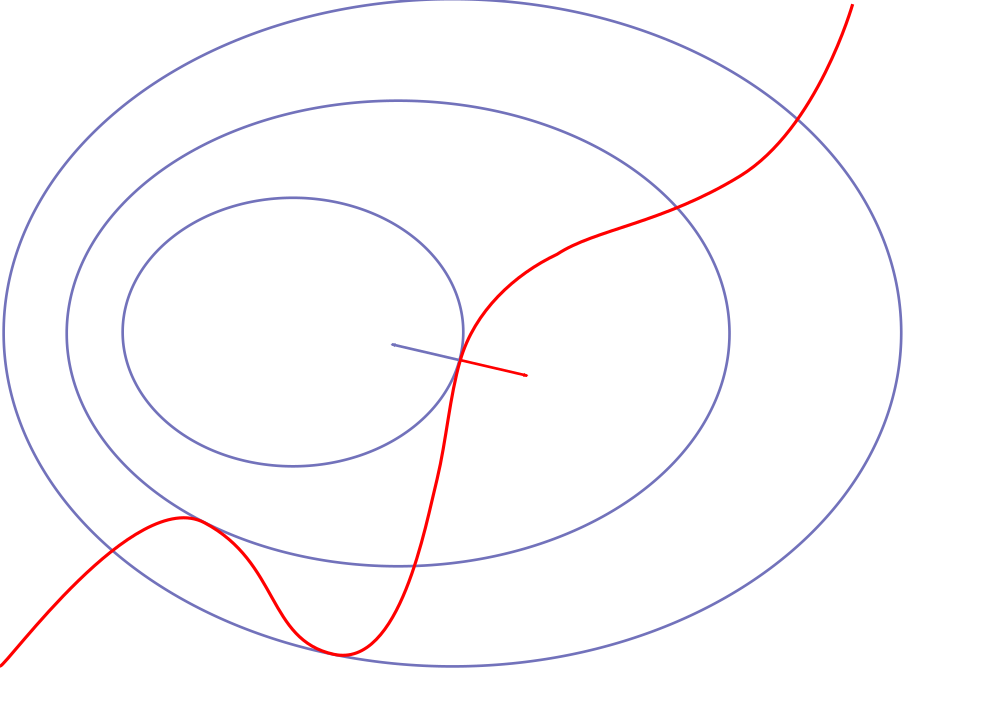
\includegraphics{lagrange.pdf}
        \caption{Extrema of \(f\) under constraint \(g\)}
    \end{center}
\end{figure}


\textbf{Problem:}
Minimise (or maximise) \(f(x,y)\) under the constraint \(g(x,y) = 0\).
\begin{itemize}
    \item At ``touching point'' the gradient vectors are parallel;
    \item I.e., \(\nabla f = \lambda \nabla g\) for some \(\lambda \in \bR\).
\end{itemize}



{Method of Lagrange's multipliers}.
If a scalar field \(f(x_1,\ldots,x_n)\) has a relative extremum when it is subject to \(m\) constraints
\[
    g_1(x_1,\ldots,x_n) = 0,
    \dots , g_m(x_1,\ldots,x_n)=0,
\]
where \(m<n\), then there exist \(m\) scalars \(\lambda_1,\ldots,\lambda_m\) such that
\[
    \nabla f = \lambda_1 \nabla g_1 + \cdots + \lambda_m \nabla g_m
\]
at the extremum point.



\begin{example*}
    Find the extrema of \(f(x,y) = xy\) subject to the constraint \(g(x,y) = x+y-1 =0\).
    \begin{itemize}
        \item \(\nabla f(x,y) = \left(\begin{smallmatrix}
                  y\\ x
              \end{smallmatrix}\right)\)
              and \(\nabla g(x,y) = \left(\begin{smallmatrix}
                  1\\ 1
              \end{smallmatrix}\right)\);
        \item  According to the Lagrange multiplier method there is \(\lambda\in \bR\) such that \(\nabla f(x,y) = \lambda \nabla g(x,y)\) at the extremum point \((x,y)\);
        \item We must solve the simultaneous equations
              \[
                  \left(\begin{smallmatrix}
                          y\\ x
                      \end{smallmatrix}\right)
                  = \lambda \left(\begin{smallmatrix}
                          1\\ 1
                      \end{smallmatrix}\right),
                  \quad g(x,y) =0;
              \]
        \item I.e.,
              \( x = \lambda, \quad
              y = \lambda, \quad
              x+y = 1;
              \)
        \item This has the solution \((x,y) = (\frac{1}{2},\frac{1}{2})\), \(f(\frac{1}{2},\frac{1}{2})= \frac{1}{4}\).
    \end{itemize}
\end{example*}


\begin{example*}
    Find the points closest and furthest from the origin on the curve defined by the intersection of the two surfaces
    \[
        x^2 - xy + y^2 - z^2 = 1
        \quad \text{and} \quad
        x^2 + y^2 = 1.
    \]
    \vspace{-1em}
    \begin{itemize}
        \item Let \(f(x,y,z) = \sqrt{x^2 + y^2 + z^2}\);
        \item Let \(g_1(x,y,z) = x^2 - xy + y^2 - z^2 - 1\),
              \(g_2(x,y,z) = x^2 + y^2 - 1\);
        \item Calculate \(\nabla f\), \(\nabla g_1\) and \(\nabla g_2\);
        \item Solve the system of 5 equations (and 5 unknowns):
              \vspace{-1em}
              \[
                  \nabla f (x,y,z) = \lambda_1 \nabla g_1(x,y,z)  + \lambda_2 \nabla g_2(x,y,z),
              \]
              \[
                  \quad g_1(x,y,z) =0,
                  \quad g_2(x,y,z) =0;
              \]
        \item Check which are closest to and which are furthest from the origin.
    \end{itemize}
\end{example*}



